\documentclass[11pt,a4paper]{article}

\usepackage[utf8]{inputenc}
\usepackage[T1]{fontenc}
\usepackage[margin=1in]{geometry}
\usepackage[table]{xcolor}
\usepackage[most]{tcolorbox}
\usepackage{hyperref}
\usepackage{tabularx}
\usepackage{booktabs}
\usepackage{tikz}
\usepackage{fancyhdr}
\usepackage{fontawesome5}
\usepackage{amsmath}

% --- Premium Typography & Spacing ---
\usepackage{mathpazo}
\usepackage{setspace}
\setstretch{1.15}

% --- Premium Section Headings ---
\usepackage{titlesec}
\titleformat{\section}
  {\normalfont\Large\bfseries\color{dpiblue}}{\thesection}{1em}{}[{\color{dpicloud}\vspace{0.2cm}\titlerule[1pt]}]
\titleformat{\subsection}
  {\normalfont\large\bfseries\color{dpiteal}}{\thesubsection}{1em}{}

% --- Premium Hyperlinks ---
\hypersetup{
    colorlinks=true,
    linkcolor=dpiblue,
    filecolor=dpiblue,      
    urlcolor=dpiteal,
    citecolor=dpiblue
}

% Custom Header Style
\pagestyle{fancy}
\setlength{\headheight}{25pt}
\fancyhf{}
\fancyhead[L]{\textbf{\color{dpiblue} DPI-LS Framework}}
\fancyhead[R]{\color{dpiblue} Measuring Execution (E)}
\fancyfoot[C]{\color{dpiblue}\textbf{Page \thepage}}
\renewcommand{\headrulewidth}{1pt}
\renewcommand{\headrule}{\hbox to\headwidth{\color{dpiblue}\leaders\hrule height \headrulewidth\hfill}}
\usetikzlibrary{shapes.geometric, arrows.meta, positioning, calc, backgrounds, fit, trees, mindmap, matrix, shadows}

% Define DPI-LS Brand Colors
\definecolor{dpiblue}{HTML}{2b3a67}
\definecolor{dpigreen}{HTML}{498467}
\definecolor{dpired}{HTML}{b0413e}
\definecolor{dpilight}{HTML}{e5f9e0}
\definecolor{dpicloud}{HTML}{f4a261}
\definecolor{dpiteal}{HTML}{318281}

% Define Custom GitHub-Style Alerts
\newtcolorbox{dpinote}[1][]{enhanced, colback=blue!5!white, colframe=dpiblue, title={\textbf{NOTE}}, fonttitle=\bfseries, attach boxed title to top left={xshift=5mm,yshift=-2mm}, #1}
\newtcolorbox{dpiimportant}[1][]{enhanced, colback=red!5!white, colframe=dpired, title={\textbf{IMPORTANT}}, fonttitle=\bfseries, attach boxed title to top left={xshift=5mm,yshift=-2mm}, #1}
\newtcolorbox{dpitip}[1][]{enhanced, colback=dpigreen!5!white, colframe=dpigreen, boxrule=0.5pt, leftrule=3pt, sharp corners, #1}

\begin{document}

\begin{titlepage}
    \pagecolor{dpiblue}
    \color{white}
    \begin{center}
        \vspace*{3cm}
        
        {\Huge \textbf{Measuring Execution}} \\[0.7cm]
        {\LARGE \textbf{Guide for the DPI-LS Project}}
        
        \vspace{2cm}
        
        {\color{dpicloud}\rule{0.5\textwidth}{1.5pt}}
        
        \vspace{2cm}
        
        {\Large \textit{Digital Performance Index --- Execution Dimension (E)}} \\[1cm]
        
        {\large Architecture, Integration \& Business Capabilities}
        
        \vfill
        
        % Stylish Geometric Cover Overlay
        \begin{tikzpicture}[remember picture, overlay]
            % Subtle watermark circles in the corners
            \fill[white, opacity=0.05] (current page.north east) circle (5cm);
            \fill[white, opacity=0.05] (current page.south west) circle (7cm);
            \fill[dpiteal, opacity=0.1] (current page.south east) circle (9cm);
            
            % Giant faded icon in the center as a watermark
            \node[font=\fontsize{150}{150}\selectfont, text=white, opacity=0.03] at (current page.center) {\faServer};
        \end{tikzpicture}
        
        \renewcommand{\arraystretch}{1.3}
        \begin{tabular}{rl}
            \textbf{Framework:} & Digital Performance Index (DPI-LS) \\
            \textbf{Dimension:} & Execution (E) --- Weight: 20\% \\
            \textbf{Version:} & 1.0 \\
            \textbf{Status:} & Architectural Reference \\
        \end{tabular}
        
        \vspace{2cm}
        
        {\color{dpicloud}\rule{0.5\textwidth}{1pt}} \\[0.5cm]
        
        {\large DPI-LS Architecture Team}
        
        \vspace*{1cm}
    \end{center}
\end{titlepage}
\pagecolor{white}
\color{black}

\tableofcontents
\newpage

\section{Executive Summary \& Introduction}

\begin{dpinote}
The \textbf{Digital Performance Index (DPI-LS)} framework quantifies AI agent performance across 7 distinct dimensions. Within this framework, the \textbf{Execution (E)} dimension tracks an agent's technical reliability and tool-calling success rate.
\end{dpinote}

As AI Agents move from chat interfaces to autonomous workflows, they rely heavily on external tools, API calls, and code execution. When an agent attempts to execute a tool (e.g., querying a database, calling an API, writing to a file), it can either succeed or fail due to hallucinations, malformed JSON, or network errors.

This document provides the architectural guidelines for measuring the \textbf{Execution} dimension. It evaluates how we track agent function calls, how we integrate these telemetry points into the DPI-LS engine, and how measuring execution directly reflects on the operational resilience of the agent.

\vspace{0.5cm}

\section{Execution Tracking Mind Map}

The following mind map outlines the core requirements of measuring AI Agent Execution within the DPI-LS framework.

\vspace{0.5cm}
\vspace{0.5cm}
\begin{center}
\resizebox{0.9\textwidth}{!}{%
\begin{tikzpicture}[
  mindmap,
  every node/.style={concept, execute at begin node=\hskip0pt, drop shadow},
  root concept/.append style={concept color=dpiblue, fill=dpiblue, line width=1ex, text=white, font=\large\bfseries},
  level 1 concept/.append style={font=\small\bfseries, level distance=5.5cm, text=white},
  level 2 concept/.append style={font=\footnotesize, level distance=3cm, text=black},
  grow cyclic
]
\node[root concept] {AI Agent \\ Execution}
  child[concept color=dpigreen, sibling angle=90] { node {Function \\ Calling}
    child[sibling angle=45] { node[fill=white] {Syntax} }
    child[sibling angle=45] { node[fill=white] {APIs} }
    child[sibling angle=45] { node[fill=white] {JSON} }
  }
  child[concept color=dpicloud, sibling angle=90] { node {Attempts}
    child[sibling angle=45] { node[fill=white] {Retries} }
    child[sibling angle=45] { node[fill=white] {Timeouts} }
    child[sibling angle=45] { node[fill=white] {Failures} }
  }
  child[concept color=dpired, sibling angle=90] { node {Methods}
    child[sibling angle=60] { node[fill=white] {Tracing} }
    child[sibling angle=60] { node[fill=white] {APM} }
  }
  child[concept color=teal, sibling angle=90] { node {Metrics}
    child[sibling angle=60] { node[fill=white] {Recovery} }
    child[sibling angle=60] { node[fill=white] {Fallbacks} }
  };
\end{tikzpicture}
}
\end{center}

\newpage

\section{The Execution Formula (How E is Calculated)}

The Execution dimension relies on a transparent mathematical formula calculated natively within the DPI-LS engine. It evaluates the agent's ability to successfully execute its planned actions.

\begin{dpiimportant}
\textbf{Formula:} $E = \frac{\text{successful\_executions}}{\text{total\_attempts}}$
\end{dpiimportant}

\begin{itemize}
    \item \textbf{total\_attempts:} The total number of times an agent tries to execute a tool, function, or API call.
    \item \textbf{successful\_executions:} The number of those attempts that return a successful 200 OK or valid operational state without crashing or failing.
\end{itemize}

\subsection{\textcolor{dpiteal}{Calculation Example}}
Suppose an AI Agent makes \textbf{14 total attempts} to use tools during a complex reasoning workflow:

\begin{table}[htbp]
\centering
\renewcommand{\arraystretch}{1.4}
\rowcolors{2}{gray!10}{white}
\small
\arrayrulecolor{gray!50}
\begin{tabularx}{\textwidth}{| >{\raggedright\arraybackslash}X >{\raggedright\arraybackslash}X >{\raggedright\arraybackslash}X >{\raggedright\arraybackslash}X |}
\hline
\textbf{Attempt Sequence} & \textbf{Status} & \textbf{Outcome} & \textbf{Recorded Success} \\
\hline
Attempts 1-10 & Success & Fetches correct records & 10 \\
Attempt 11 & Failure & Hallucinates missing parameter & 0 \\
Attempt 12 & Success & Self-corrects and retries & 1 \\
Attempt 13 & Failure & External service times out & 0 \\
Attempt 14 & Success & Succeeds on second try & 1 \\
\hline
\end{tabularx}
\end{table}

\begin{dpitip}
\textbf{\textcolor{dpigreen}{\faLightbulb\ TIP \quad The Math:}}
\begin{align*}
\text{successful\_executions} &= 12 \\
\text{total\_attempts} &= 14 \\
E &= \frac{12}{14} \\
\textbf{Final E-Score} &= \mathbf{0.857}
\end{align*}
\end{dpitip}

\vspace{0.5cm}
\begin{center}
\resizebox{0.9\textwidth}{!}{%
\begin{tikzpicture}[
    node distance=1.5cm,
    action_clean/.style={rectangle, draw=dpigreen, fill=dpigreen!10, thick, text width=2cm, align=center, minimum height=1cm, rounded corners},
    action_fail/.style={rectangle, draw=dpired, fill=red!10, thick, text width=2cm, align=center, minimum height=1cm, rounded corners},
    arrow/.style={-{Stealth[scale=1.2]}, thick},
    label/.style={font=\footnotesize\itshape}
]

\node[action_clean] (a1) {Attempt 1-10\\ \textbf{Success}};
\node[action_fail, right=of a1] (a2) {Attempt 11\\ \textbf{Failure}};
\node[action_clean, right=of a2] (a3) {Attempt 12\\ \textbf{Success}};
\node[action_fail, right=of a3] (a4) {Attempt 13\\ \textbf{Failure}};
\node[action_clean, right=of a4] (a5) {Attempt 14\\ \textbf{Success}};

\draw[arrow] (a1) -- (a2);
\draw[arrow] (a2) -- (a3);
\draw[arrow] (a3) -- (a4);
\draw[arrow] (a4) -- (a5);

\node[rectangle, draw=dpiblue, fill=blue!5, thick, text width=4.5cm, align=center, minimum height=1.5cm, below=of a3, yshift=-1cm] (score) {\textbf{Final Score Calculation} \\ $E = \frac{12}{14} = \mathbf{0.857}$};

\draw[arrow, dashed, draw=dpired] (a2.south) |- (score.west);
\draw[arrow, dashed, draw=dpired] (a4.south) |- (score.east);

\end{tikzpicture}
}
\end{center}

\begin{dpitip}
\textbf{The Math:}\\
$E = 12 / 14 = 0.857$\\
\textbf{Final E-Score = 0.857}
\end{dpitip}

An agent with an execution score of \texttt{1.0} flawlessly calls APIs and tools without needing to self-correct or retry. A lower score indicates the agent is struggling with syntax, hallucinations in function calling, or interacting with unstable external environments.

\newpage

\section{Core Integration Architecture}

To reflect an agent's current Execution score on the DPI-LS dashboard, the agent framework must hook into the DPI-LS telemetry ingestion API to report tool attempts and their statuses.

\vspace{0.5cm}
\vspace{0.5cm}
\begin{center}
\resizebox{0.9\textwidth}{!}{%
\begin{tikzpicture}[
    node distance=1.5cm and 2cm,
    block/.style={rectangle, rounded corners, draw=dpiblue, fill=dpilight, thick, text width=3.5cm, align=center, minimum height=1.2cm, drop shadow},
    server/.style={rectangle, rounded corners, top color=dpigreen!20, bottom color=dpigreen!50, draw=dpigreen, thick, text width=3.5cm, align=center, minimum height=1.2cm, drop shadow},
    alert/.style={diamond, aspect=2, draw=dpired, fill=red!10, thick, text width=2.5cm, align=center, drop shadow},
    arrow/.style={-{Stealth[scale=1.2]}, thick},
    box/.style={rectangle, draw=gray, dashed, thick, inner sep=0.5cm}
]

% Nodes
\node[block] (agent) {AI Agent Framework};
\node[block, above=of agent] (user) {User Request};

\node[block, right=of agent, xshift=1.5cm] (tool) {External Tool / API};
\node[block, below=of tool] (callback) {Telemetry Callback};
\node[alert, below=of callback] (status) {Status Code?};

\node[server, right=of status, xshift=1cm] (api) {DPI-LS Ingestion API};
\node[server, below=of api] (db) {DPI-LS Database};
\node[server, below=of db] (engine) {Scoring Engine};
\node[server, right=of engine] (dashboard) {Live Dashboard};

% Subgraphs
\begin{scope}[on background layer]
    \node[box, fill=gray!5, fit=(user) (agent) (tool), label={[font=\bfseries]above:Client Environment}] (client) {};
    \node[box, fill=blue!5, fit=(callback) (status), label={[font=\bfseries]above:Telemetry Layer}] (eval) {};
    \node[box, fill=green!5, fit=(api) (db) (engine) (dashboard), label={[font=\bfseries]above:DPI-LS Server}] (server) {};
\end{scope}

% Arrows
\draw[arrow] (user) -- (agent);
\draw[arrow] (agent) to[bend left] node[above, font=\footnotesize] {1. Try Tool Call} (tool);
\draw[arrow, dashed] (tool) to[bend left] node[below, font=\footnotesize] {2. Success/Fail} (agent);

\draw[arrow] (agent) |- node[above, font=\footnotesize] {3. Emit Call Status} (callback);
\draw[arrow] (callback) -- node[right, font=\footnotesize] {4. Log Event} (status);

\draw[arrow] (status) -- node[above, font=\footnotesize] {5. Push Log} (api);
\draw[arrow] (api) -- node[right, font=\footnotesize] {6. Update} (db);
\draw[arrow] (db) -- node[right, font=\footnotesize] {7. Recalc E-Score} (engine);
\draw[arrow] (engine) -- node[above, font=\footnotesize] {8. Update UI} (dashboard);

\end{tikzpicture}
}
\end{center}

\vspace{0.5cm}

\section{Various Possible Ways for Measuring Execution (E)}

The DPI-LS framework is highly flexible, providing multiple avenues for capturing the E-score depending on the agent framework and infrastructure. The matrix below summarizes the supported methodologies:

\vspace{0.3cm}
\begin{center}
\resizebox{0.65\textwidth}{!}{
\begin{tikzpicture}[
    node distance=2cm and 2.5cm,
    center_node/.style={circle, top color=dpiblue!10, bottom color=dpiblue!30, draw=dpiblue, thick, text width=2.5cm, align=center, minimum height=2.5cm, font=\bfseries, drop shadow},
    native_node/.style={rectangle, rounded corners, top color=dpigreen!10, bottom color=dpigreen!30, draw=dpigreen, thick, text width=2.8cm, align=center, minimum height=1cm, drop shadow},
    direct_node/.style={rectangle, rounded corners, top color=orange!10, bottom color=orange!30, draw=dpicloud, thick, text width=2.8cm, align=center, minimum height=1cm, drop shadow},
    apm_node/.style={rectangle, rounded corners, top color=red!10, bottom color=red!30, draw=dpired, thick, text width=2.8cm, align=center, minimum height=1cm, drop shadow},
    arrow/.style={-{Stealth[scale=1.2]}, thick, draw=gray}
]

\node[center_node] (dpils) {DPI-LS \\ Execution Engine};

% Native
\node[native_node, above left=of dpils, yshift=-0.5cm, xshift=1cm] (langchain) {LangChain};
\node[native_node, above right=of dpils, yshift=-0.5cm, xshift=-1cm] (llamaindex) {LlamaIndex};

% Direct
\node[direct_node, left=of dpils] (openai) {OpenAI Functions};
\node[direct_node, right=of dpils] (bedrock) {AWS Bedrock Tools};

% APM
\node[apm_node, below left=of dpils, yshift=1cm, xshift=1cm] (datadog) {Datadog APM};
\node[apm_node, below right=of dpils, yshift=1cm, xshift=-1cm] (dynatrace) {Dynatrace};

% Connections
\draw[arrow] (langchain) -- (dpils);
\draw[arrow] (llamaindex) -- (dpils);
\draw[arrow] (openai) -- (dpils);
\draw[arrow] (bedrock) -- (dpils);
\draw[arrow] (datadog) -- (dpils);
\draw[arrow] (dynatrace) -- (dpils);

\end{tikzpicture}
}
\end{center}
\vspace{0.5cm}

\subsection{Execution Integration Matrix}

\begin{table}[htbp]
\centering
\renewcommand{\arraystretch}{1.4}
\rowcolors{2}{gray!10}{white}
\small
\arrayrulecolor{gray!50}
\begin{tabularx}{\textwidth}{| >{\raggedright\arraybackslash}X >{\raggedright\arraybackslash}X >{\raggedright\arraybackslash}p{3cm} >{\raggedright\arraybackslash}X |}
\hline
\rowcolor{dpicloud!30} \textbf{Execution Data} & \textbf{What It Measures} & \textbf{Source System} & \textbf{Actual Data Comes From} \\
\hline
Agent graph tracing \& debugging & Tool execution attempts and errors & LangSmith & LangSmith SDK pushes traces to webhook \\
Framework-native callback tracking & Tool execution attempts and errors in Python & LangChain & Custom BaseTracer injected into execution \\
Query pipeline telemetry & Query engine success rate & LlamaIndex & OTel Exporter to DPI-LS API \\
LLM-native function resolution & Successful JSON payload generation & OpenAI API & Parsing completion response \texttt{finish\_reason} \\
Application performance monitoring & Low-level API network success & Datadog & HTTP 4xx/5xx logs correlated to agent traces \\
Standardized OTel LLM telemetry & GenAI Semantic Conventions spans & OpenLLMetry & Traceloop SDK exports \\
Full-stack trace analytics & Asynchronous agent execution graphs & Langfuse & Langfuse SDK exports \\
OpenInference AI observability & LLM tool span evaluation & Arize Phoenix & Phoenix OTLP exports \\
Enterprise span logging \& evaluation & Tool execution trace logging & Braintrust & \texttt{braintrust} SDK logging \\
Chain-of-thought error tracking & Errors in multi-step workflows & Galileo & \texttt{galileo-observe} SDK \\
Open-source LLM tracing & Trace capture and debugging & Opik (by Comet) & Opik Python SDK / REST API \\
Multi-agent session tracking & Multi-agent execution loops & AgentOps & Native hooks into CrewAI / AutoGen \\
Gateway-level API routing logs & Intercepted HTTP headers at the edge & Helicone / Portkey & AI Proxy routing \\
Code-level function decoration & Wrapped Python functions & Custom App Code & \texttt{@dpi\_track\_execution} decorator \\
\hline
\end{tabularx}
\end{table}

\vspace{0.5cm}

\subsection{Execution Integration Decision Tree}

\vspace{0.3cm}
\begin{center}
\resizebox{0.85\textwidth}{!}{
\begin{tikzpicture}[
    >=stealth, thick,
    decision/.style={diamond, aspect=2, draw=gray, fill=dpilight, text width=2.5cm, align=center, inner sep=1pt},
    native/.style={rectangle, rounded corners, draw=white, fill=dpigreen, text=white, text width=3cm, align=center, inner sep=4pt},
    third/.style={rectangle, rounded corners, draw=white, fill=dpiblue, text=white, text width=3cm, align=center, inner sep=4pt},
    cloud/.style={rectangle, rounded corners, draw=gray, fill=dpicloud, text width=3cm, align=center, inner sep=4pt}
]

% Column 1
\node[decision] (start) at (0, 0) {Agent\\Framework?};

% Column 2
\node[decision] (custom) at (4, 0) {Custom\\Built?};
\node[native] (langchain) at (4, -4) {LangChain\\Callbacks};
\node[native] (llamaindex) at (4, -6) {LlamaIndex\\OTel Exporter};

% Column 3
\node[decision] (llm) at (8, 0) {LLM API\\Provider?};
\node[decision] (apm) at (8, -4) {Enterprise\\APM?};

% Column 4
\node[cloud] (openai) at (12, 0) {OpenAI\\finish\_reason};
\node[cloud] (anthropic) at (12, -2) {Anthropic\\stop\_reason};

\node[third] (datadog) at (12, -4) {Datadog HTTP};
\node[third] (dynatrace) at (12, -6) {Dynatrace APM};
\node[third] (openllmetry) at (12, -8) {OpenLLMetry};


% Connections
\draw[->] (start) -- node[above, font=\footnotesize] {No} (custom);
\draw[->] (start) |- node[near start, left, font=\footnotesize] {Yes: LC} (langchain);
\draw[->] (start) |- node[near start, left, font=\footnotesize] {Yes: LI} (llamaindex);

\draw[->] (custom) -- node[above, font=\footnotesize] {Yes} (llm);
\draw[->] (custom) |- node[near start, left, font=\footnotesize] {Yes} (apm);

\draw[->] (llm) -- node[above, font=\footnotesize] {OpenAI} (openai);
\draw[->] (llm) |- node[near start, left, font=\footnotesize] {Anthropic} (anthropic);

\draw[->] (apm) -- node[above, font=\footnotesize] {Datadog} (datadog);
\draw[->] (apm) |- node[near start, left, font=\footnotesize] {Dynatrace} (dynatrace);
\draw[->] (apm) |- node[near start, left, font=\footnotesize] {OTel} (openllmetry);

\end{tikzpicture}
}
\end{center}
\vspace{0.5cm}

\subsection{Native Agent Framework Integrations}


\subsubsection*{LangSmith}
\begin{itemize}
    \item \textbf{What it is:} The premier observability platform built by LangChain to track, debug, and monitor complex agentic workflows.
    \item \textbf{How can we integrate and use this for DPI-LS project:} LangSmith captures the complete execution flow of an agent, including every tool invocation, retrieval step, and reasoning logic. If a tool fails, LangSmith natively logs the exception, the exact inputs that caused it, and the latency.
    \item \textbf{How to wire it up:}
    \begin{enumerate}
        \item Enable tracing in the environment via \texttt{LANGCHAIN\_TRACING\_V2=true}.
        \item Use the LangSmith SDK to automatically capture all agent loops.
        \item Configure LangSmith automation rules to POST failed tool executions directly to the DPI-LS webhook.
    \end{enumerate}
\end{itemize}

\subsubsection*{LangChain \& LangGraph}
\begin{itemize}
    \item \textbf{What it is:} The most popular open-source frameworks for building complex agentic architectures and stateful workflows.
    \item \textbf{How can we integrate and use this for DPI-LS project:} By implementing a custom \texttt{BaseCallbackHandler}, DPI-LS can hook directly into the \texttt{on\_tool\_start}, \texttt{on\_tool\_end}, and \texttt{on\_tool\_error} events. This allows native, precise tracking of exactly when an agent attempts a tool and whether it succeeded or crashed natively in Python.
    \item \textbf{How to wire it up:}
    \begin{enumerate}
        \item Create a \texttt{DPIExecutionCallbackHandler(BaseCallbackHandler)} class.
        \item Implement \texttt{on\_tool\_error} to dispatch a failure payload to the DPI-LS Webhook.
        \item Pass the callback handler into the Agent Executor initialization.
    \end{enumerate}
\end{itemize}

\vspace{0.2cm}\hrule\vspace{0.2cm}

\subsubsection*{LlamaIndex}
\begin{itemize}
    \item \textbf{What it is:} A data framework specifically designed for connecting custom data sources to LLMs for RAG and agentic querying.
    \item \textbf{How can we integrate and use this for DPI-LS project:} LlamaIndex natively supports OpenTelemetry (OTel). If a query pipeline or tool execution fails, the OTel spans immediately register the exception.
    \item \textbf{How to wire it up:}
    \begin{enumerate}
        \item Configure the \texttt{OpenTelemetrySpanHandler} in the LlamaIndex dispatcher.
        \item Route the OTel exporter to the DPI-LS ingestor endpoint.
        \item Filter spans by type \texttt{TOOL\_CALL} and aggregate successes vs failures for the E-Score.
    \end{enumerate}
\end{itemize}

\vspace{0.2cm}\hrule\vspace{0.2cm}

\subsection{Direct API \& Cloud Provider Integrations}

\subsubsection*{OpenAI Function Calling API}
\begin{itemize}
    \item \textbf{What it is:} Native tool use capabilities built directly into OpenAI models like GPT-4o.
    \item \textbf{How can we integrate and use this for DPI-LS project:} For lightweight agents not using heavy frameworks, DPI-LS can monitor the raw API responses. If an agent outputs \texttt{finish\_reason: "tool\_calls"} but fails to provide a valid JSON schema matching the registered functions, it counts as an execution failure.
\end{itemize}

\vspace{0.2cm}\hrule\vspace{0.2cm}

\subsection{OpenTelemetry \& Third-Party Observability}

\subsubsection*{OpenLLMetry (by Traceloop)}
\begin{itemize}
    \item \textbf{What it is:} An open-source observability framework built on OpenTelemetry, specifically designed to track LLM execution and agent tool calling using GenAI Semantic Conventions.
    \item \textbf{How can we integrate and use this for DPI-LS project:} OpenLLMetry automatically instruments agent workflows (like LangChain or LlamaIndex) and treats the agent's entire execution flow as a distributed trace. If an agent's tool call crashes, the exception is recorded as a child span.
    \item \textbf{How to wire it up:}
    \begin{enumerate}
        \item Install the \texttt{traceloop-sdk} and initialize it in the application entry point.
        \item Use \texttt{@workflow} and \texttt{@task} decorators on custom tool functions to ensure they are captured as individual spans.
        \item Export the telemetry data to the DPI-LS backend using a standard OTel exporter, allowing DPI-LS to penalize the E-score upon detecting tool-call error spans.
    \end{enumerate}
\end{itemize}

\vspace{0.2cm}\hrule\vspace{0.2cm}

\subsubsection*{Langfuse}
\begin{itemize}
    \item \textbf{What it is:} An open-source, full-stack LLM engineering platform that focuses on comprehensive trace analytics, prompt management, and evaluation.
    \item \textbf{How can we integrate and use this for DPI-LS project:} Langfuse excels at visualizing complex, multi-turn agent execution graphs. It natively integrates with frameworks like LangChain, tracking the exact latency, cost, and tool-call sequence of every execution.
    \item \textbf{How to wire it up:}
    \begin{enumerate}
        \item Add the \texttt{Langfuse} callback handler to your agent loop.
        \item Map Langfuse's concept of a "Trace" to the DPI-LS Session ID.
        \item Route Langfuse's webhooks or export its datasets into the DPI-LS ingestion API to calculate the E-score.
    \end{enumerate}
\end{itemize}

\vspace{0.2cm}\hrule\vspace{0.2cm}

\subsubsection*{Arize Phoenix}
\begin{itemize}
    \item \textbf{What it is:} An open-source AI observability platform that leverages the OpenInference standard to trace LLM applications using OpenTelemetry.
    \item \textbf{How can we integrate and use this for DPI-LS project:} Phoenix provides deep visibility into retrieval (RAG) and tool-calling performance. If an agent calls a tool and the context retrieved is irrelevant or the execution fails, Phoenix captures this as an OpenInference span.
    \item \textbf{How to wire it up:}
    \begin{enumerate}
        \item Instrument the agent application with the \texttt{openinference-instrumentation} library.
        \item Point the OTLP exporter to a Phoenix server (or directly to a compatible DPI-LS collector).
        \item Analyze the trace spans for \texttt{ToolCall} events marked with \texttt{StatusCode.ERROR}.
    \end{enumerate}
\end{itemize}

\vspace{0.2cm}\hrule\vspace{0.2cm}

\subsection{AI Gateway \& Proxy Integrations}

\subsubsection*{Helicone \& Portkey}
\begin{itemize}
    \item \textbf{What it is:} Open-source AI gateways that act as a proxy layer between your application and the LLM providers.
    \item \textbf{How can we integrate and use this for DPI-LS project:} Gateways provide zero-code observability. Because they intercept the raw HTTP requests, they can instantly capture malformed tool-calls, timeouts, and token costs without requiring you to install heavy tracing SDKs in your agent logic.
    \item \textbf{How to wire it up:}
    \begin{enumerate}
        \item Change your agent's LLM Base URL to point to the Helicone or Portkey proxy instance.
        \item The gateway captures the \texttt{finish\_reason} and full tool-call payload.
        \item Route the gateway's webhooks directly to the DPI-LS Engine to record E-score failures.
    \end{enumerate}
\end{itemize}

\vspace{0.2cm}\hrule\vspace{0.2cm}

\subsection{Agent-Specific Observability}

\subsubsection*{AgentOps}
\begin{itemize}
    \item \textbf{What it is:} An open-source observability platform purpose-built for multi-agent frameworks (like CrewAI, AutoGen, and PraisonAI) rather than generic LLM calls.
    \item \textbf{How can we integrate and use this for DPI-LS project:} AgentOps captures the "session replay" and causal chain of why an agent selected a tool. It natively tracks "Agent Loops" and "Time Travel Debugging", making it perfect for complex execution failures.
    \item \textbf{How to wire it up:}
    \begin{enumerate}
        \item Initialize \texttt{agentops.init()} at the start of your multi-agent script.
        \item AgentOps automatically wraps framework tool executions.
        \item Use the AgentOps REST API to pull failed execution graphs and push them to the DPI-LS metrics database.
    \end{enumerate}
\end{itemize}

\vspace{0.2cm}\hrule\vspace{0.2cm}


\subsection{Enterprise APM Integrations}

\subsubsection*{Datadog / Dynatrace}
\begin{itemize}
    \item \textbf{What it is:} Deep infrastructure monitoring platforms that track every network request, CPU spike, and HTTP status code in your cloud environment.
    \item \textbf{How can we integrate and use this for DPI-LS project:} Agents often fail because the \textit{external API} they are trying to call is down (e.g. 504 Gateway Timeout, 500 Internal Server Error). APMs catch these network failures automatically.
    \item \textbf{How to wire it up:}
    \begin{enumerate}
        \item Correlate APM traces with Agent Session IDs.
        \item When Datadog detects a \texttt{5xx} error triggered by the agent's service, it fires a Webhook to DPI-LS.
        \item The DPI-LS engine records this as an Execution Failure and penalizes the E-Score.
    \end{enumerate}
\end{itemize}


\newpage

\section{Business Scenarios: Real-World Execution Failures}

To illustrate the value of tracking tool execution natively within DPI-LS, consider the following enterprise scenarios where an agent attempts to utilize external functions.

When a tool fails, the agent must either self-correct or fail gracefully. The DPI-LS system tracks these transitions. The state diagram below visualizes this exact flow:

\vspace{0.5cm}
\vspace{0.5cm}
\begin{center}
\resizebox{0.8\textwidth}{!}{%
\begin{tikzpicture}[
    node distance=1cm and 2cm,
    state/.style={rectangle, rounded corners, draw=dpiblue, fill=blue!5, thick, text width=3cm, align=center, minimum height=1cm},
    alert/.style={rectangle, rounded corners, draw=dpired, fill=red!10, thick, text width=3.5cm, align=center, minimum height=1cm},
    action/.style={rectangle, rounded corners, draw=dpigreen, fill=green!10, thick, text width=3.5cm, align=center, minimum height=1cm},
    arrow/.style={-{Stealth[scale=1.2]}, thick},
    box/.style={rectangle, draw=gray, dashed, thick, inner sep=0.5cm}
]

\node[state] (deploy) {Deploy Agent};
\node[state, below=of deploy] (reasoning) {Reasoning};
\node[state, right=of reasoning, xshift=1cm] (attempt) {Tool Call Attempt};

\begin{scope}[on background layer]
    \node[box, fill=gray!5, fit=(reasoning) (attempt), label={[font=\bfseries, text=dpiblue]above:Agent Active}] (agentbox) {};
\end{scope}

\draw[arrow] (deploy) -- (reasoning);
\draw[arrow] (reasoning) -- node[above, font=\footnotesize] {Generate JSON} (attempt);

\node[action, below=of attempt, xshift=-2.5cm, yshift=-0.5cm] (execsuccess) {Execution Success};
\node[alert, below=of attempt, xshift=2.5cm, yshift=-0.5cm] (execfail) {Execution Failure};

\draw[arrow] (attempt) -- node[left, font=\footnotesize] {Valid Payload} (execsuccess);
\draw[arrow] (attempt) -- node[right, font=\footnotesize] {Malformed / 404} (execfail);

\node[alert, below=of execfail] (alertnode) {Log Attempt = Failed};
\node[alert, below=of alertnode] (score) {E-Score Dropped};

\begin{scope}[on background layer]
    \node[box, fill=red!5, draw=dpired, fit=(alertnode) (score), label={[font=\bfseries, text=dpired]above:Failure Handled}] (failbox) {};
\end{scope}

\draw[arrow] (execfail) -- (alertnode);
\draw[arrow] (alertnode) -- (score);

\node[state, fill=blue!10, right=of execfail, xshift=1cm] (selfcorrect) {Self-Correction Loop};
\draw[arrow] (execfail) -- node[above, font=\footnotesize] {LLM Fixes Syntax} (selfcorrect);
\draw[arrow, dashed] (selfcorrect) |- node[right, font=\footnotesize] {Retry Call} (attempt);

\draw[arrow] (execsuccess) -- node[left, font=\footnotesize] {Return Result} (reasoning);

\node[state, fill=red!20, draw=red, below=of selfcorrect, yshift=-1.5cm] (breaker) {Circuit Breaker: Max Retries};
\draw[arrow] (execfail) to[bend left=20] (breaker);

\end{tikzpicture}
}
\end{center}

\subsection*{Scenario 1: The Hallucinated Syntax (Malformed JSON)}

\textbf{1. The Risk Event:}\\
An autonomous data-entry agent attempts to write a record to a database, but the LLM hallucinates a parameter that doesn't exist in the tool's schema.
\begin{itemize}
    \item \textbf{Agent Intent:} \textit{"I will now insert the customer record using the \texttt{insert\_db} tool."}
    \item \textbf{Agent Payload:} \texttt{\{ "customer\_id": 123, "email": "test@test.com", "imaginary\_field": true \}}
\end{itemize}

\textbf{2. Automated Detection (How E is Detected):}\\
The agent's framework intercepts the call and attempts to validate the payload against the Pydantic schema. It throws a \texttt{ValidationError} because \texttt{imaginary\_field} does not exist. The tool call fails entirely.

\textbf{3. Integration \& Score Downgrade:}\\
\begin{itemize}
    \item \textbf{Endpoint Hit:} The tracing callback registers the failure and sends a payload to the DPI-LS backend.
    \item \textbf{Score Updated:} The DPI-LS scoring engine logs \textbf{1 failed attempt}. The agent's Execution (E) score drops. 
    \item \textbf{Outcome:} The agent might receive the error message in its prompt and try again, but the initial failure remains permanently logged against its E-score.
\end{itemize}

\subsection*{Scenario 2: The Unstable External API (Network Timeout)}

\textbf{1. The Risk Event:}\\
A financial forecasting agent successfully formats its JSON payload and calls an external stock-pricing API, but the external API is currently down.

\textbf{2. Automated Detection (How E is Detected):}\\
The HTTP request hangs for 10 seconds and throws a \texttt{TimeoutError}. Even though the agent did nothing wrong syntactically, the execution attempt failed.

\textbf{3. Integration \& Score Downgrade:}\\
\begin{itemize}
    \item \textbf{Endpoint Hit:} The Datadog APM integration catches the \texttt{504 Gateway Timeout} and pushes a failure event to DPI-LS.
    \item \textbf{Score Updated:} The DPI-LS engine registers \textbf{1 failed attempt}, downgrading the E-score.
\end{itemize}

\subsection*{Scenario 3: The Seamless Self-Correction}

\textbf{1. The Risk Event:}\\
An agent is asked to write a Python script and execute it in a sandbox. It writes the script, but forgets to import the \texttt{json} module.

\textbf{2. Automated Detection (How E is Detected):}\\
The Python sandbox tool returns the \texttt{NameError}. The DPI-LS ingestion API logs this as \textbf{1 failed attempt}.

\textbf{3. Integration \& Recovery:}\\
\begin{itemize}
    \item \textbf{Self-Correction:} The agent reads the \texttt{NameError}, realizes its mistake, adds \texttt{import json}, and tries again.
    \item \textbf{Score Updated:} The second attempt is successful. The DPI-LS engine logs \textbf{1 successful attempt}.
    \item \textbf{Outcome:} The final tally for this task is 1 success and 1 failure ($E = 1/2 = 0.50$). The agent completed the task, but the execution tracking proves it was inefficient and wasted compute cycles to get there.
\end{itemize}

\vspace{0.5cm}

\section{Business Capabilities}

By meticulously tracking the Execution dimension, organizations unlock several operational capabilities:

\begin{itemize}
    \item \textbf{Self-Correction Visibility:} By looking at the ratio of attempts to successes, engineers can see how often an agent is forced to "retry" and "self-correct". An agent that succeeds on the 3rd try still gets the job done, but it is wasting compute and latency.
    \item \textbf{Model Selection Optimization:} Different LLMs have varying levels of proficiency in generating strict JSON or adhering to complex tool schemas. The E-score provides a direct, quantifiable metric to compare how well GPT-4o executes tools compared to Claude 3.5 Sonnet or open-source models.
    \item \textbf{Flaky Tool Identification:} If multiple agents have low E-scores when interacting with a specific internal API, the telemetry will highlight that the \textit{tool} is likely flaky or poorly documented in its system prompt, rather than the agent being unintelligent.
\end{itemize}

\vspace{0.5cm}

\section{Conclusion \& Next Steps}

\begin{dpiimportant}
The Execution (E) dimension strips away the subjective nature of LLM outputs and focuses strictly on \textbf{operational reliability}. Can the agent format a payload correctly? Can it handle network exceptions? Does it crash?
\end{dpiimportant}

By integrating execution callbacks directly into your agent frameworks and piping them into the DPI-LS engine, you gain absolute clarity into the technical competence of your autonomous systems.

\textbf{Next Steps:}
\begin{enumerate}
    \item \textbf{Define Webhooks:} Ensure the DPI-LS execution API (\texttt{/webhooks/execution}) is active.
    \item \textbf{Configure Callbacks:} Install \texttt{LangChain} or \texttt{LlamaIndex} callback handlers in the agent framework to automatically push tool statistics.
    \item \textbf{Monitor Dashboard:} Observe the live UI to pinpoint failing API calls or syntactical hallucinations in real-time.
\end{enumerate}

\end{document}
